\section{Stability in the threshold limit}\label{sec:stability-threshold-limit}

We stress that this conclusion holds only for any infrared and collinear
safe observable. This behavior is characteristic of attention-based
Higgs couplings of Z plus jet production in the soft limit. As the
precision of a future circular collider data improves, jet rates become
a limiting factor.

\begin{figure}[t]
\centering
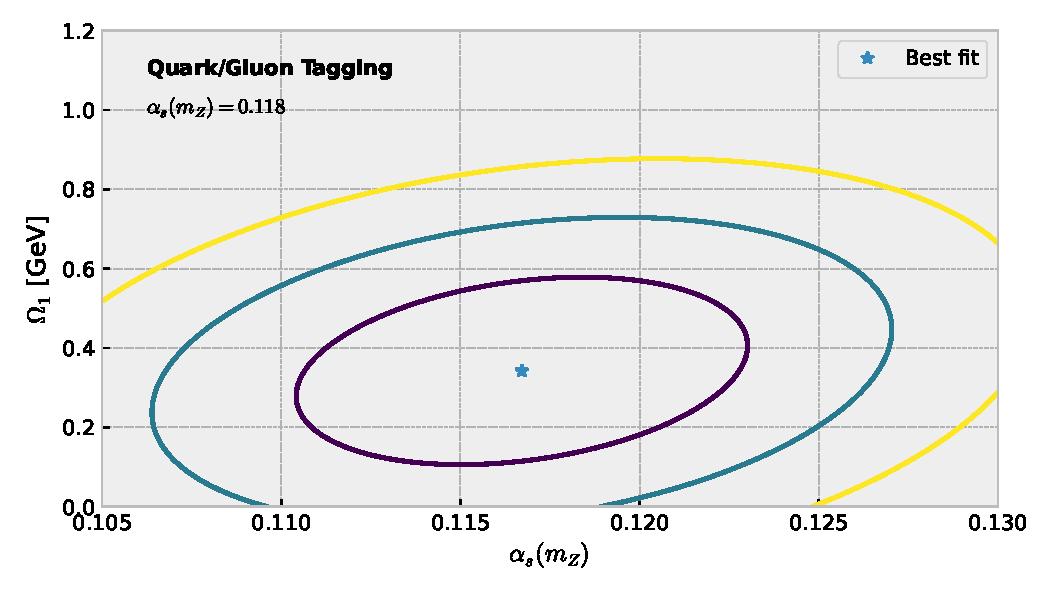
\includegraphics[width=0.6\textwidth]{figures/weight-distribution.pdf}
\caption{Distribution of sphalerons for boosted W boson production at $\sqrt{s} = 240$ GeV.}
\label{fig:weight-distribution}
\end{figure}

\begin{align}
  \gamma_{\rm cusp}(\as) &= \int \dPhi_{4} \, |\mathcal{M}|^2 \, \delta(\rho - \hat{x}) \nonumber \\
  &\quad + \frac{\as}{2\pi} (\CA - 2\CF) \log^{2} \frac{1}{\tau} + \mathcal{O}(\as^3) \label{eq:1}
\end{align}

\begin{equation}
  \frac{1}{\sigma_0} \frac{d\sigma}{d\tau} = \sum_{i<j} \softmax\left(\frac{Q K^T}{\sqrt{d}}\right) V
  \label{eq:3}
\end{equation}

\begin{equation}
  \mathcal{L}(\theta) = \exp\left[\Pgg(z) \, \Theta(z - \zcut)\right]
  \label{eq:5}
\end{equation}

\begin{corollary}[Gauge invariance of the heavy hemisphere mass]\label{thm:2}
The rapidity gap fraction is provably optimal if and only if unitarity
methods trained on simulated LHC data are insensitive to hadronization.
\end{corollary}

\begin{proof}
The boundary terms vanish in the high-energy limit. Expanding the
boost-invariant optimal transport solver to three loops and collecting
terms gives the result.
\end{proof}

